\documentclass[UTF8]{ctexart}
\usepackage{lmodern}
\usepackage{amsmath}
\usepackage{graphicx}
\usepackage{float}%提供float浮动环境
\usepackage{booktabs}%提供命令\toprule、\midrule、\bottomrule
\usepackage{geometry}

\geometry{a4paper,left=2cm,right=2cm,top=2cm,bottom=2cm}

\title{{电子技术基础实验} \\ \textbf{实验六\ 波形发生器的设计与实现
}}
\author{\\\textbf{祝尔乐}
        \\\textbf{未央-电01}
        }
\date{\textbf{\today}}

\begin{document}
\maketitle

\section*{一.实验目的}

\subsection*{1、熟悉运算放电器工作原理}
\subsection*{2、熟悉波形发生器的工作原理}
\subsection*{3、熟悉电路仿真与调试}

\section*{二.实验内容}

\subsection*{1、基于运放设计并实现一种正弦波发生电路,调节相关电路参数得到三种
频率下的波形}

本实验中我们采用文氏桥选频电路和负反馈运放电路组成的正弦波发生器,
调整电路参数,得到多种频率、振幅的正弦波。

仿真结果如图:

\begin{figure}[H]
        \centering
        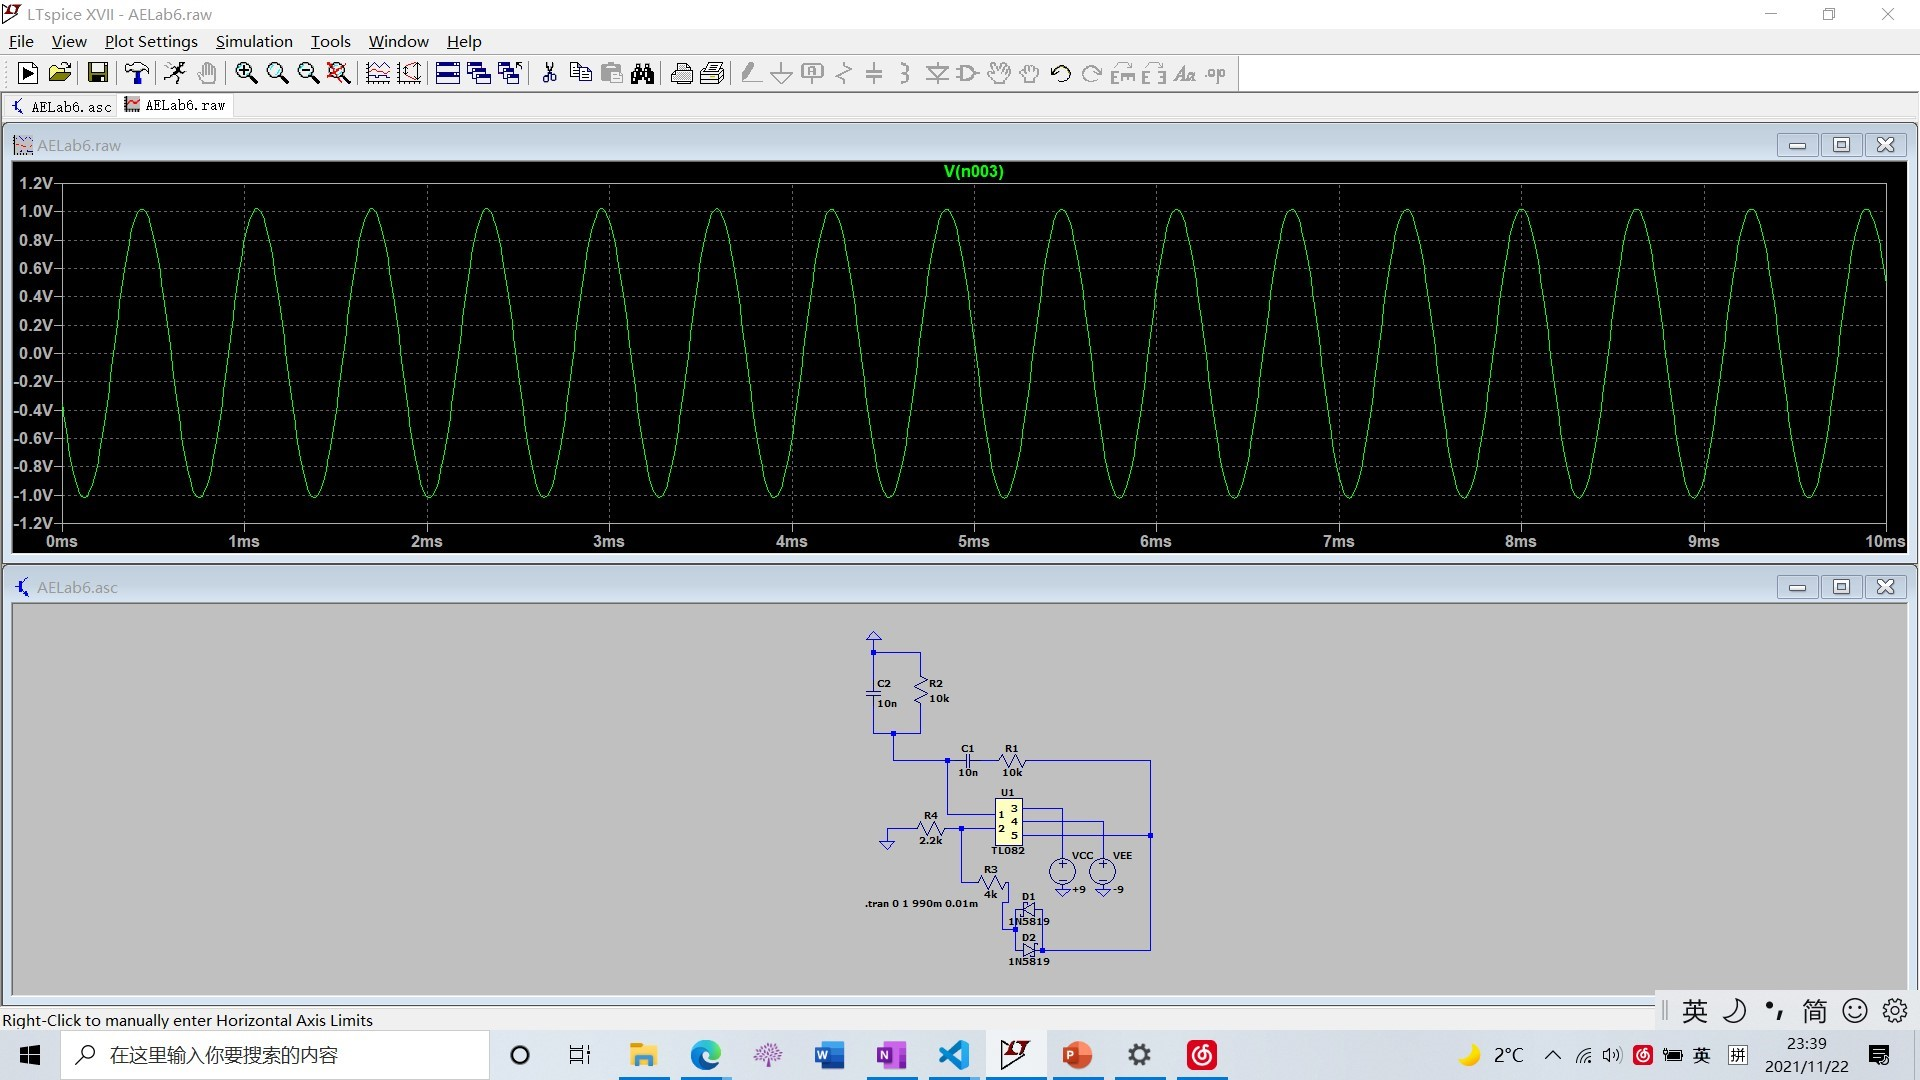
\includegraphics[width = 0.5\textwidth]{1-1-10k-10n.jpg}
        \caption{$R = 20k \Omega, C = 10nF, R_3 = 2.2 k \Omega$}
\end{figure}

\begin{figure}[H]
        \centering
        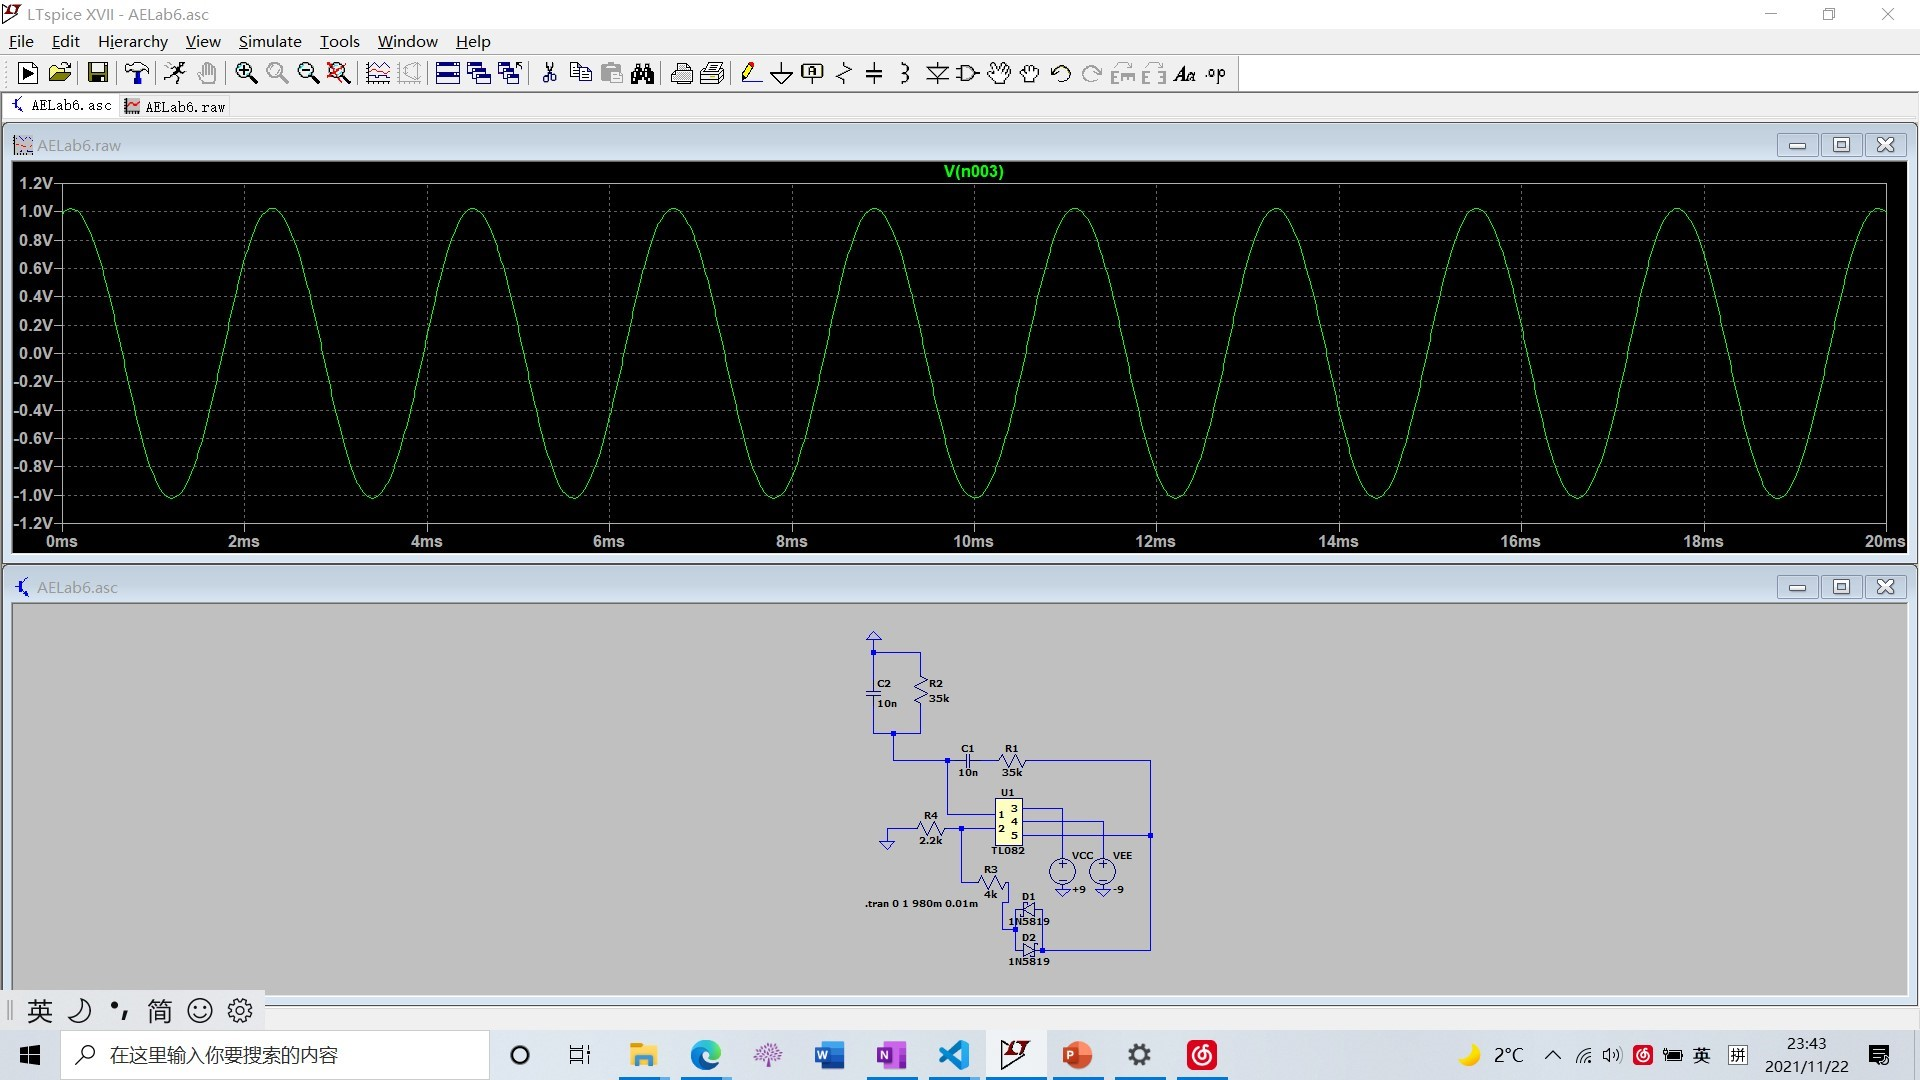
\includegraphics[width = 0.5\textwidth]{1-1-35k-10n.jpg}
        \caption{$R = 35k \Omega, C = 10nF, R_3 = 2.2 k \Omega$}
\end{figure}

\begin{figure}[H]
        \centering
        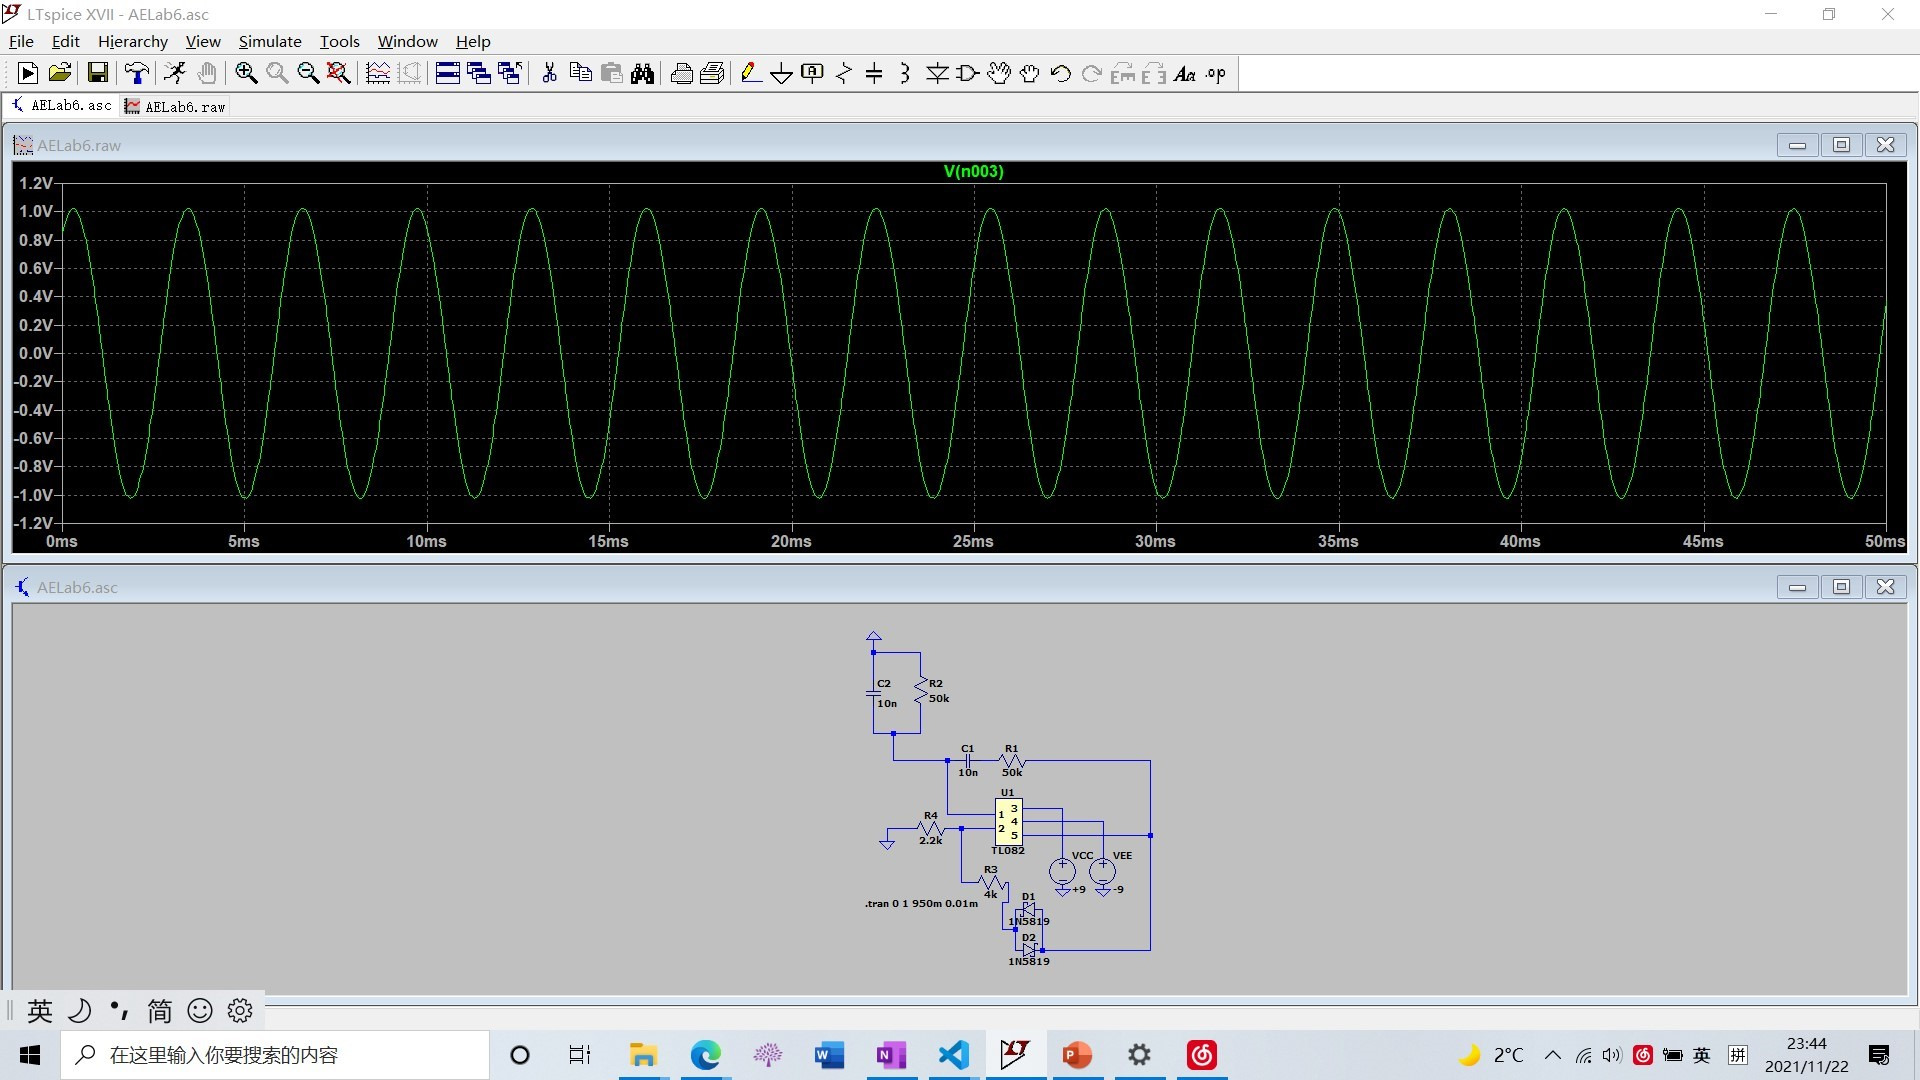
\includegraphics[width = 0.5\textwidth]{1-1-50k-10n.jpg}
        \caption{$R = 50k \Omega, C = 10nF, R_3 = 2.2 k \Omega$}
\end{figure}

\begin{figure}[H]
        \centering
        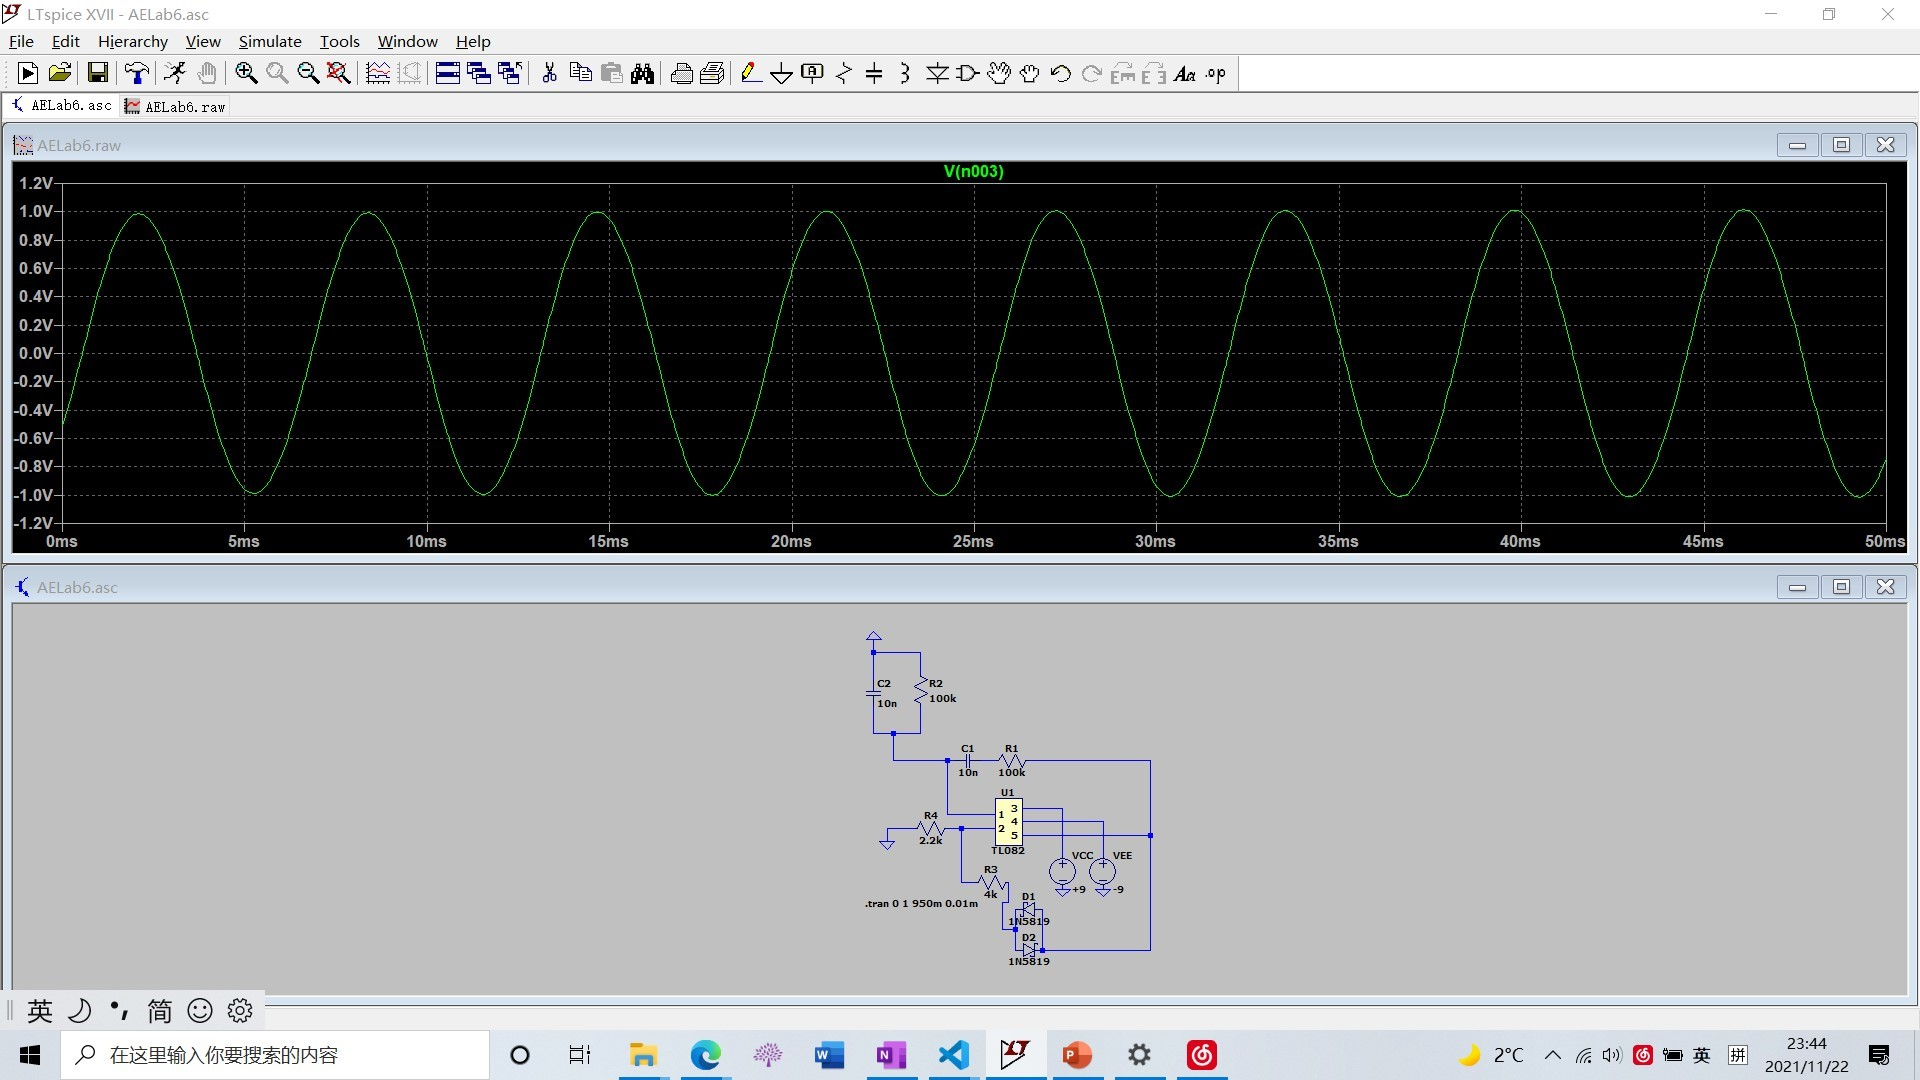
\includegraphics[width = 0.5\textwidth]{1-1-100k-10n.jpg}
        \caption{$R = 100k \Omega, C = 10nF, R_3 = 2.2 k \Omega$}
\end{figure}

\begin{figure}[H]
        \centering
        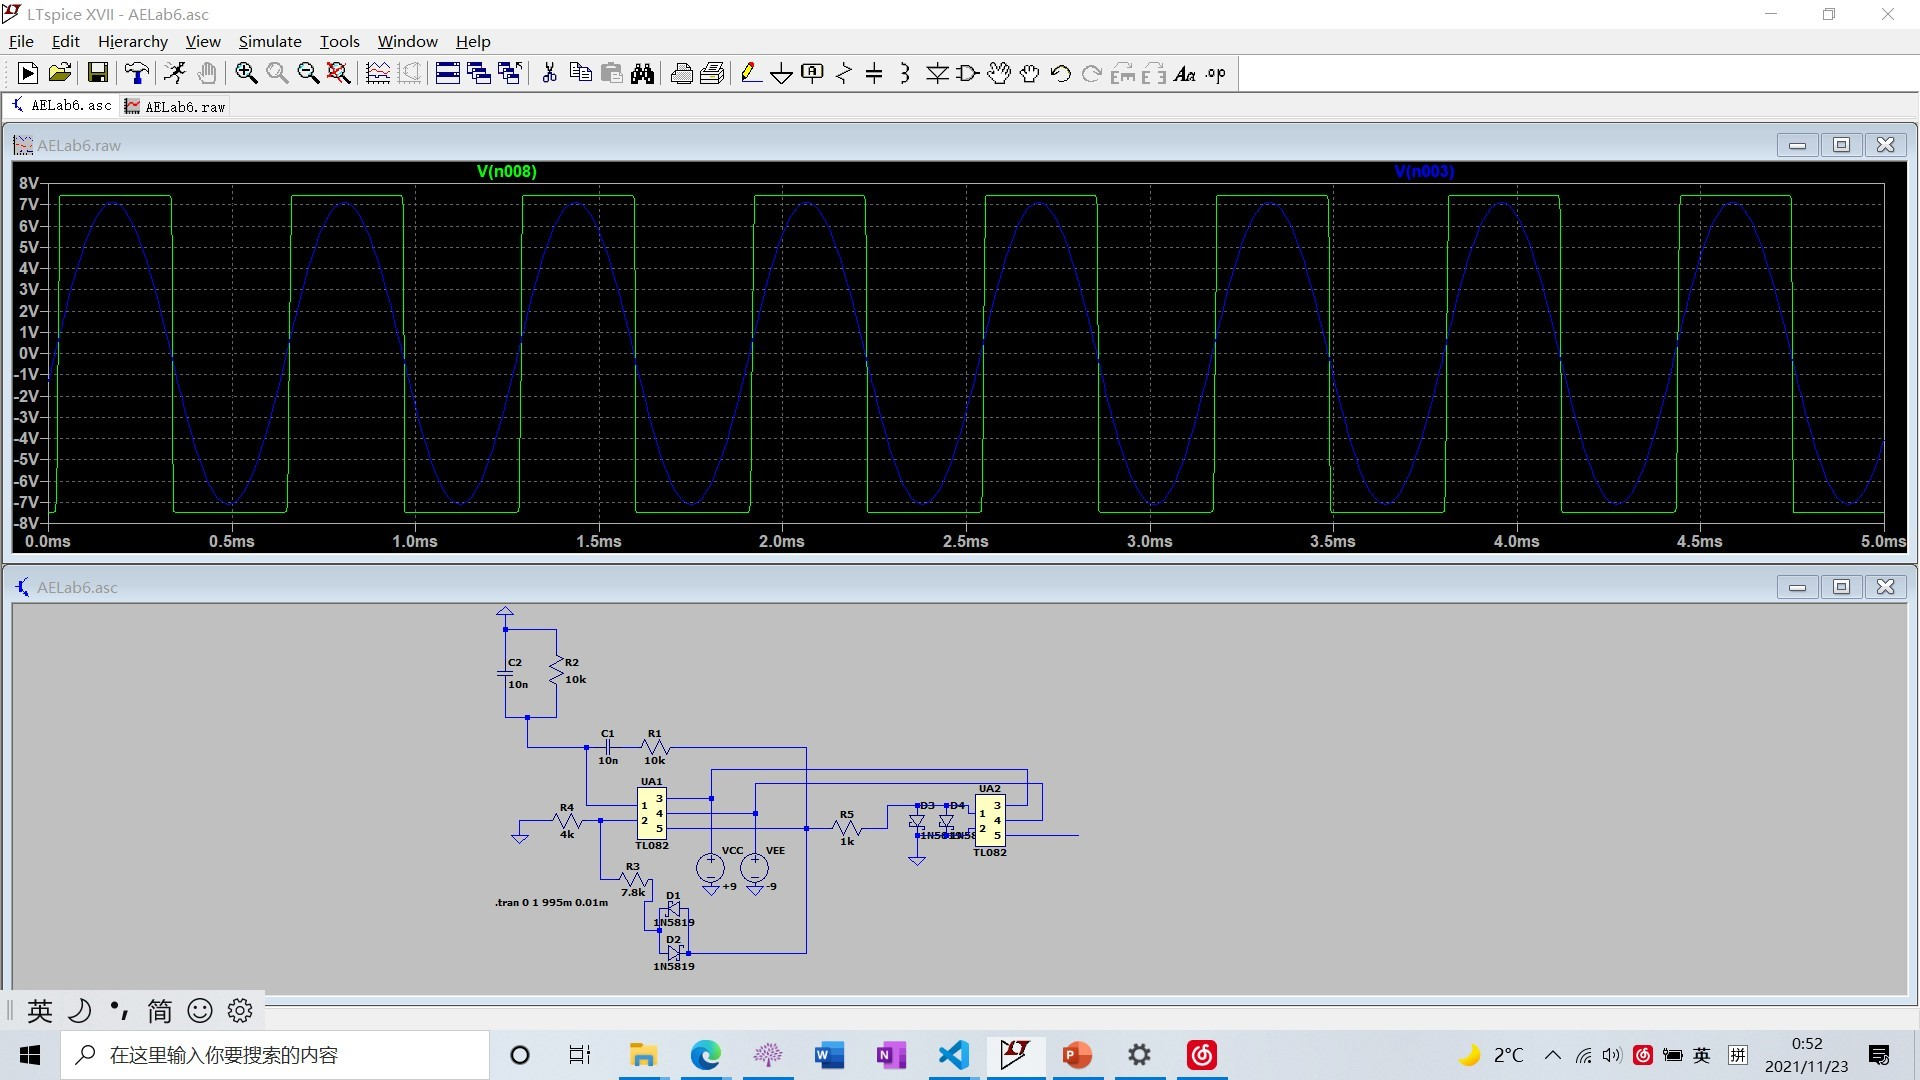
\includegraphics[width = 0.5\textwidth]{1-1-10k-10n-4.jpg}
        \caption{$R = 10k \Omega, C = 10nF, R_3 = 4 k \Omega$}
\end{figure}

\begin{figure}[H]
        \centering
        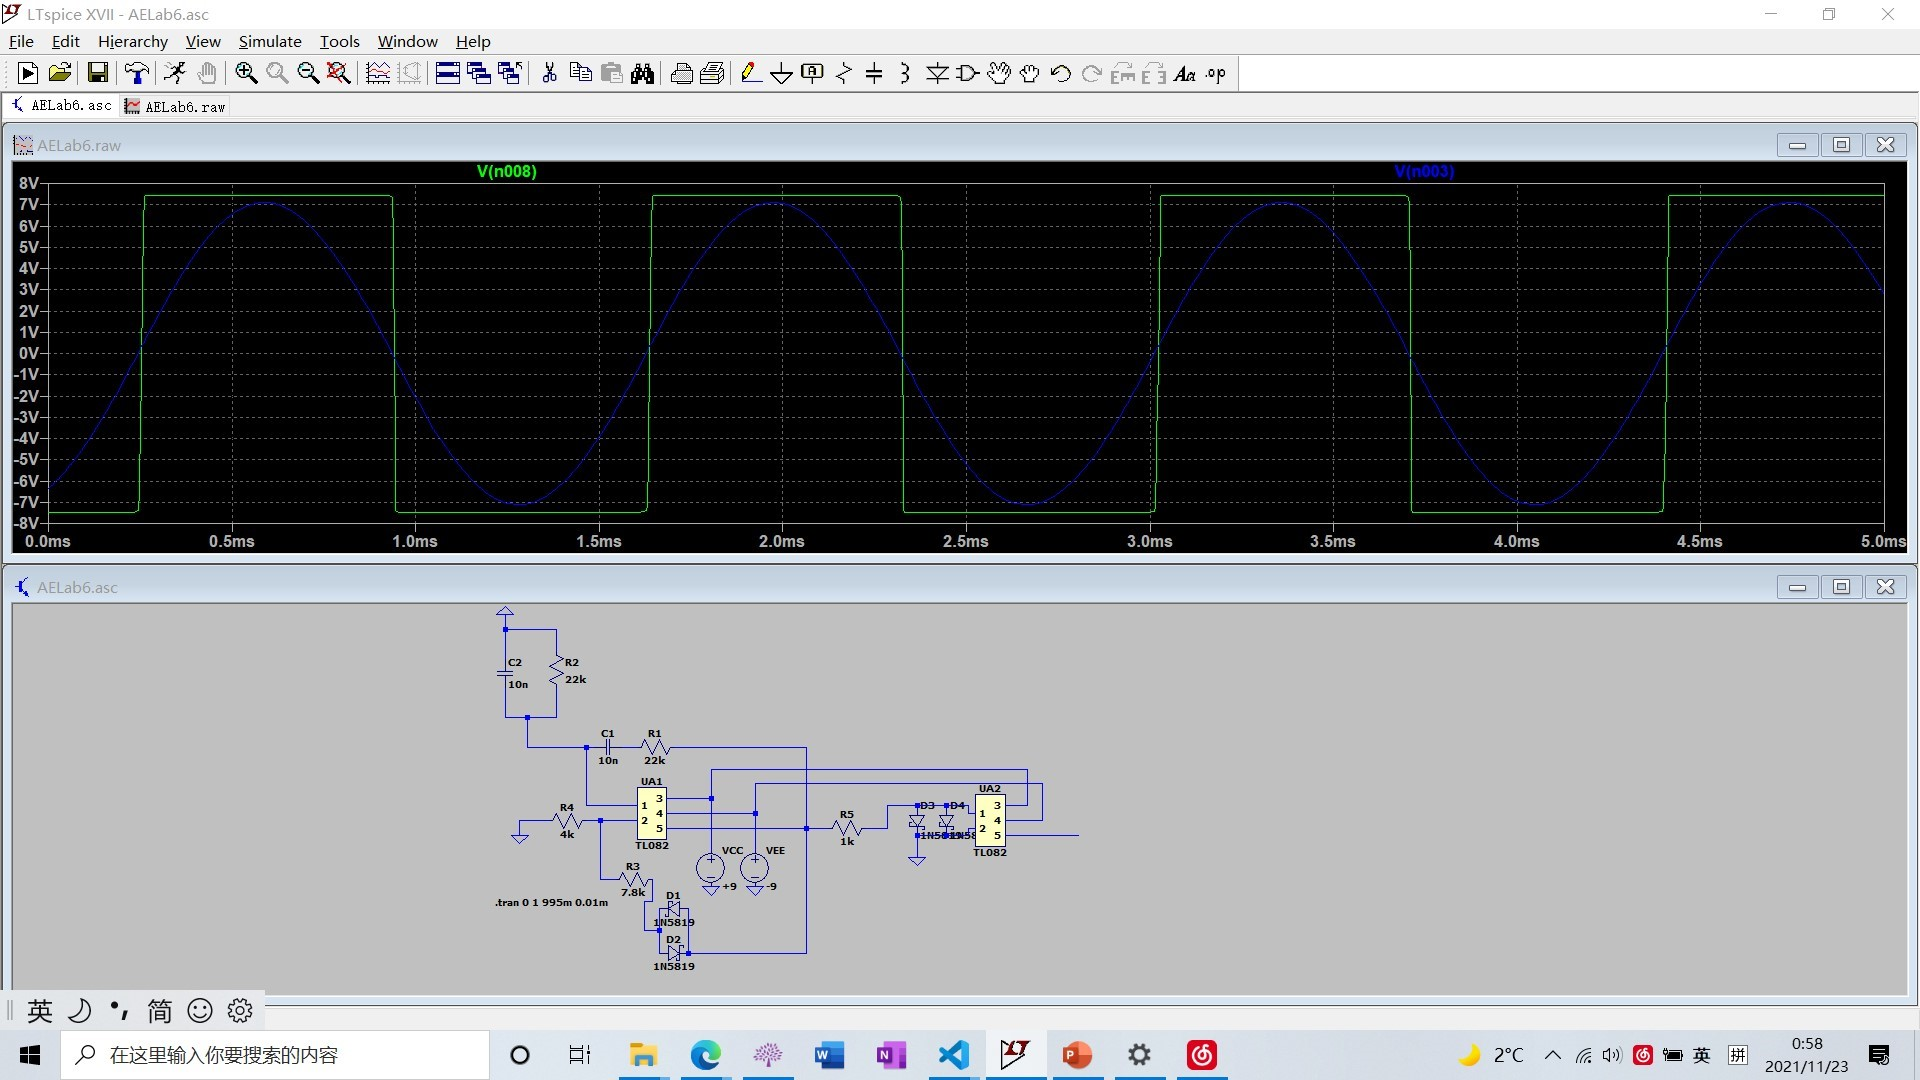
\includegraphics[width = 0.5\textwidth]{1-1-22k-10n-4.jpg}
        \caption{$R = 22k \Omega, C = 10nF, R_3 = 4 k \Omega$}
\end{figure}

\begin{figure}[H]
        \centering
        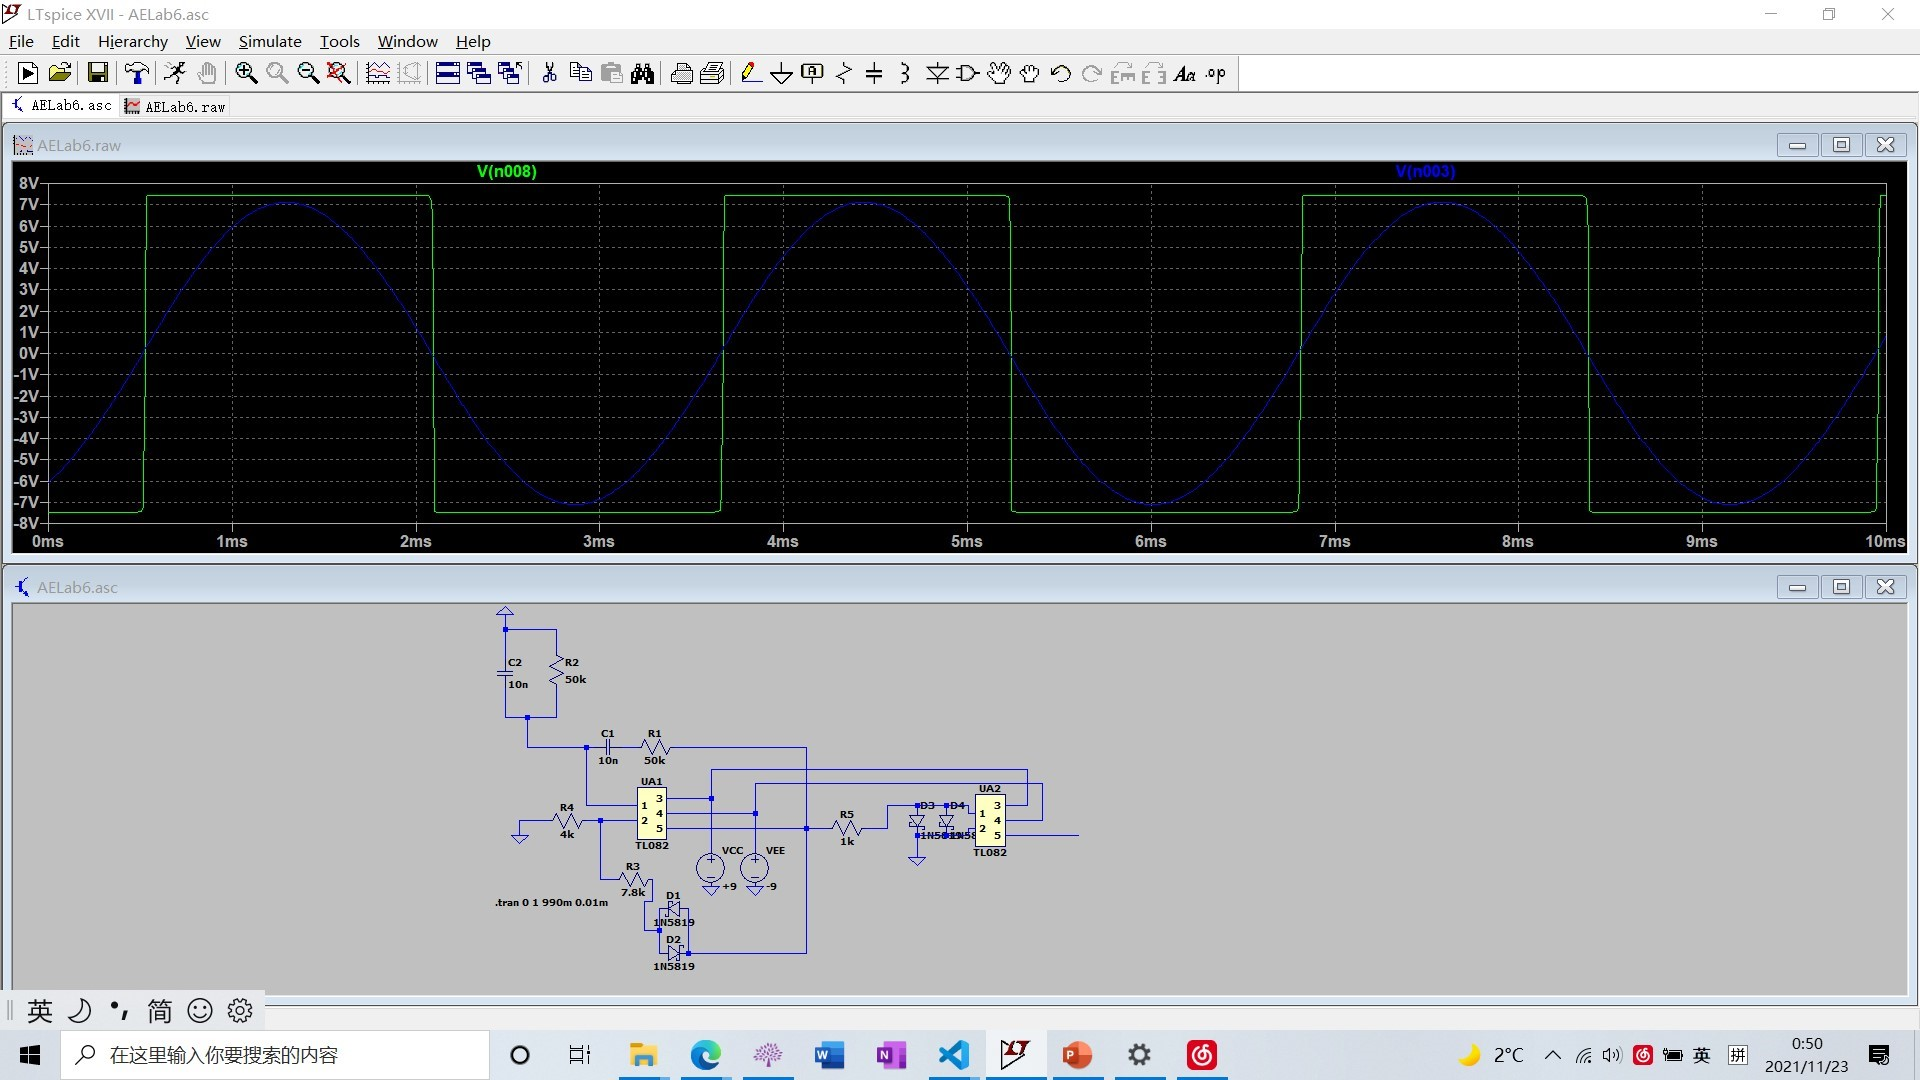
\includegraphics[width = 0.5\textwidth]{1-1-50k-10n-4.jpg}
        \caption{$R = 50k \Omega, C = 10nF, R_3 = 4 k \Omega$}
\end{figure}

实际搭建电路,令$R_3 = 4k \Omega, R_4 = 7.8 k\Omega$。

调整文氏桥$R = 10k \Omega, 22 k\Omega, 35 k\Omega, C = 10nF$,则可以得到三种频率的正弦波。
利用$f = \frac{1}{2 \pi R C}$可得三种$R、C$对应的频率为$1.59kHz, 723.4Hz, 454.7Hz$。

搭建电路图如下:

\begin{figure}[H]
        \centering
        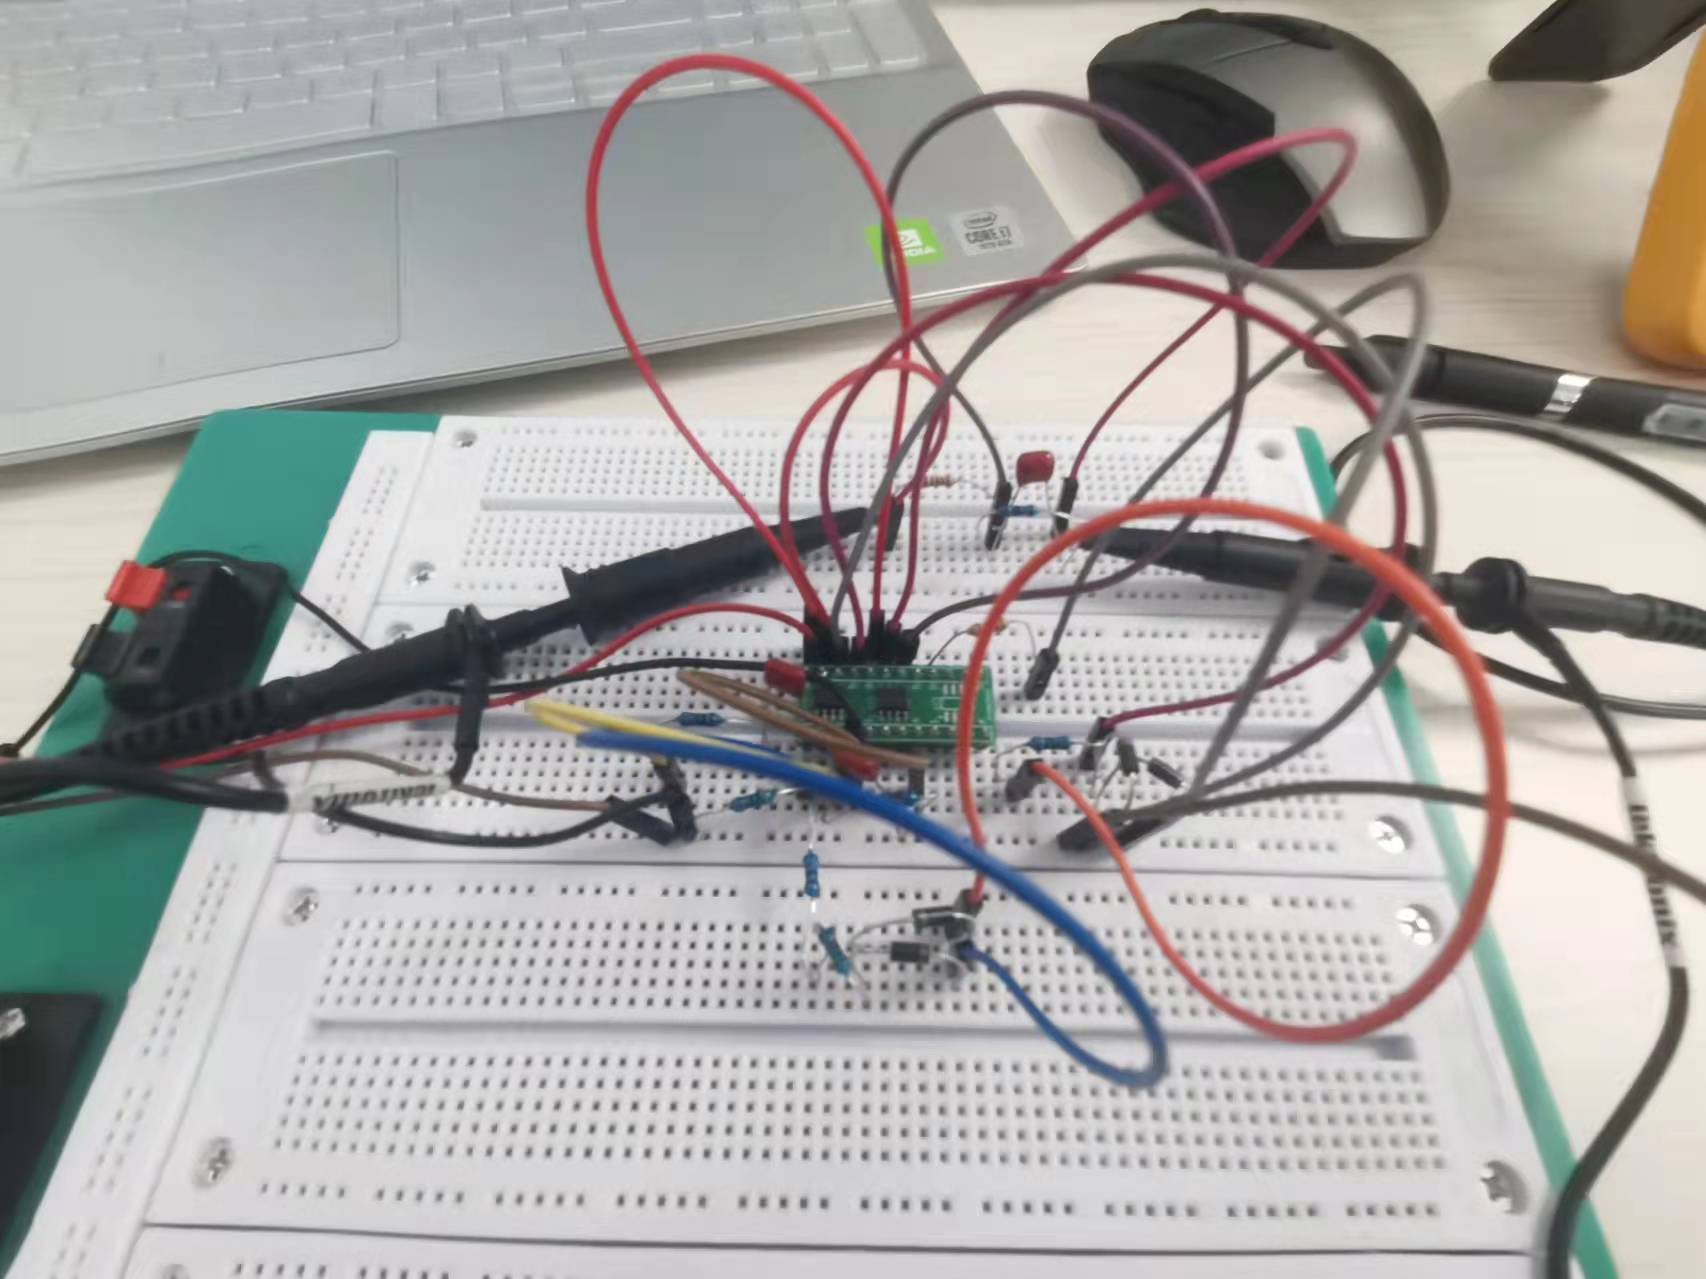
\includegraphics[width = 0.5\textwidth]{1-1-r.jpg}
        \caption{文史桥正弦波发生器}
\end{figure}

在三个$R$下,观察到正弦波波形:

\begin{figure}[H]
        \centering
        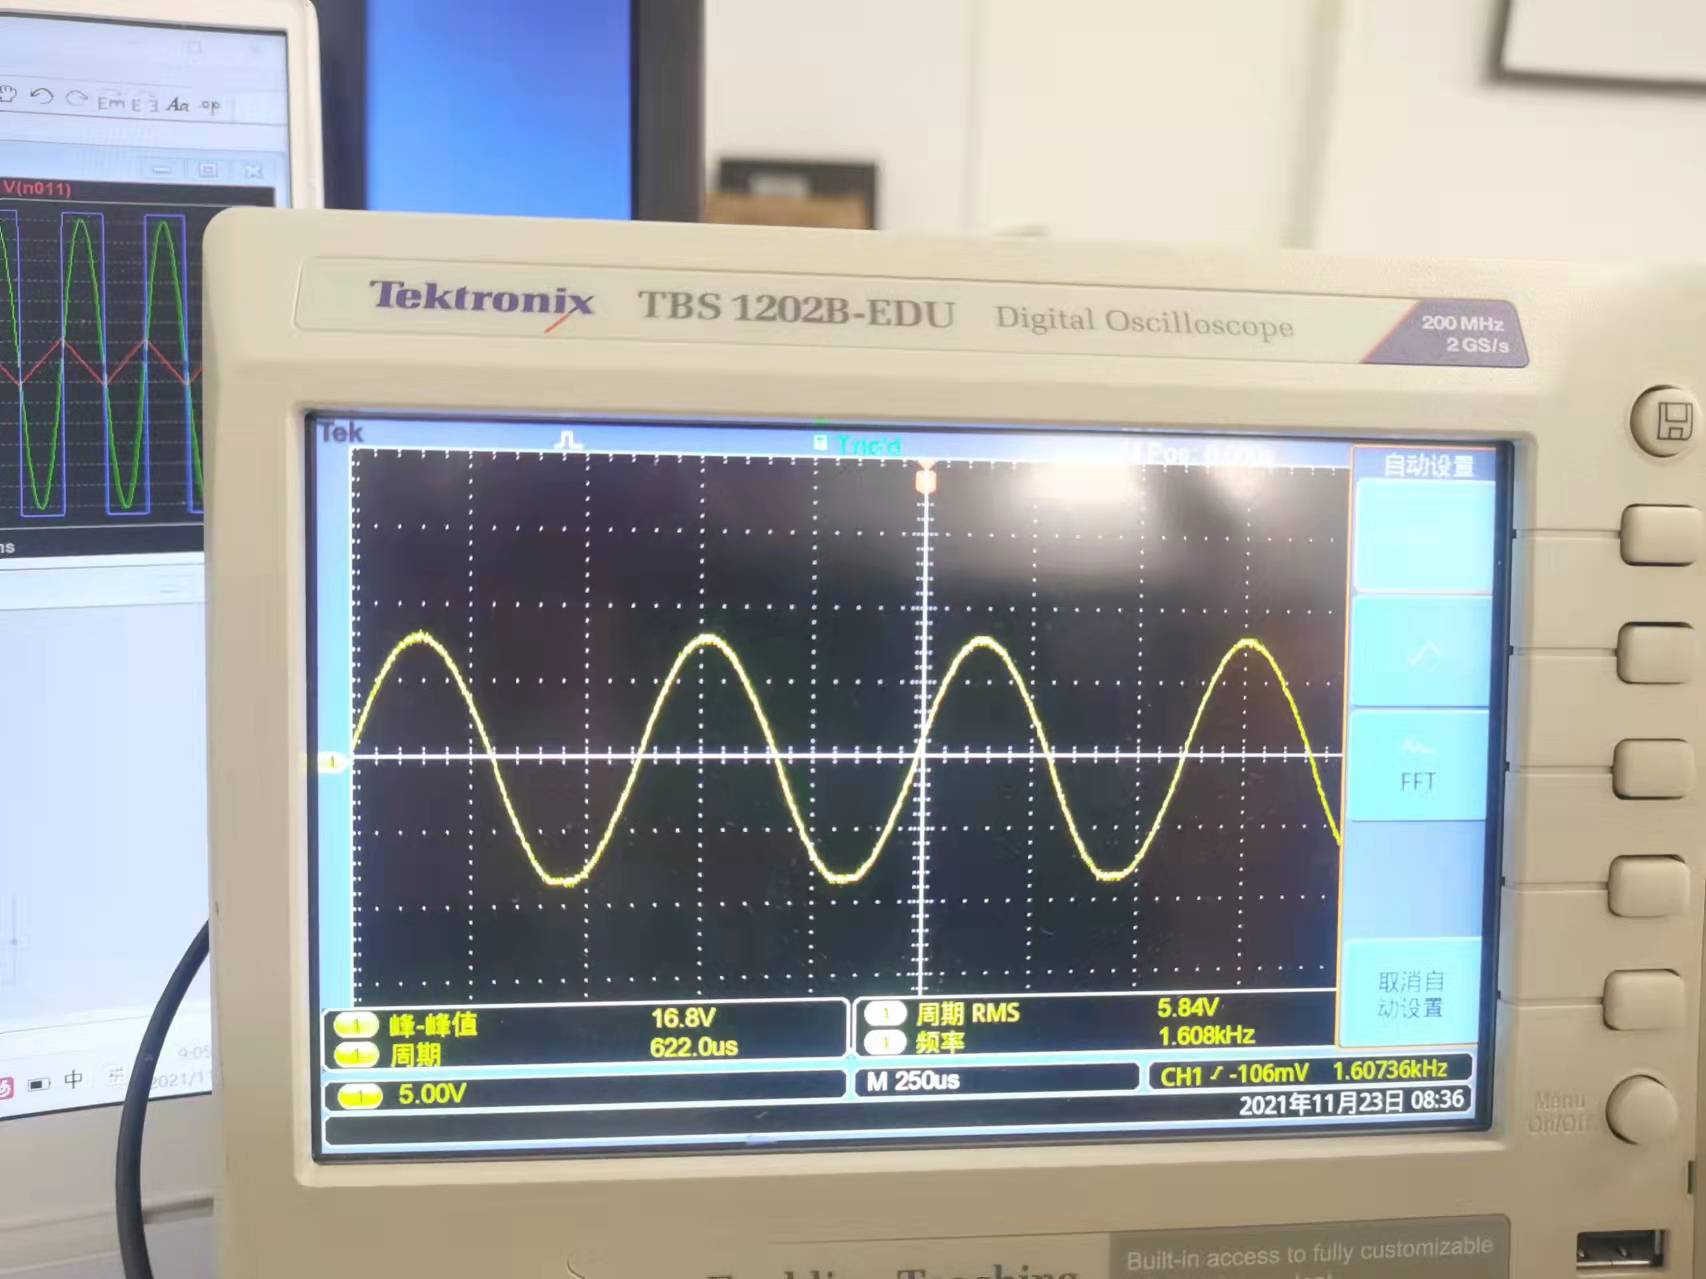
\includegraphics[width = 0.5\textwidth]{1-1-10k-r.jpg}
        \caption{$R=10k \Omega$}
\end{figure}
\begin{figure}[H]
        \centering
        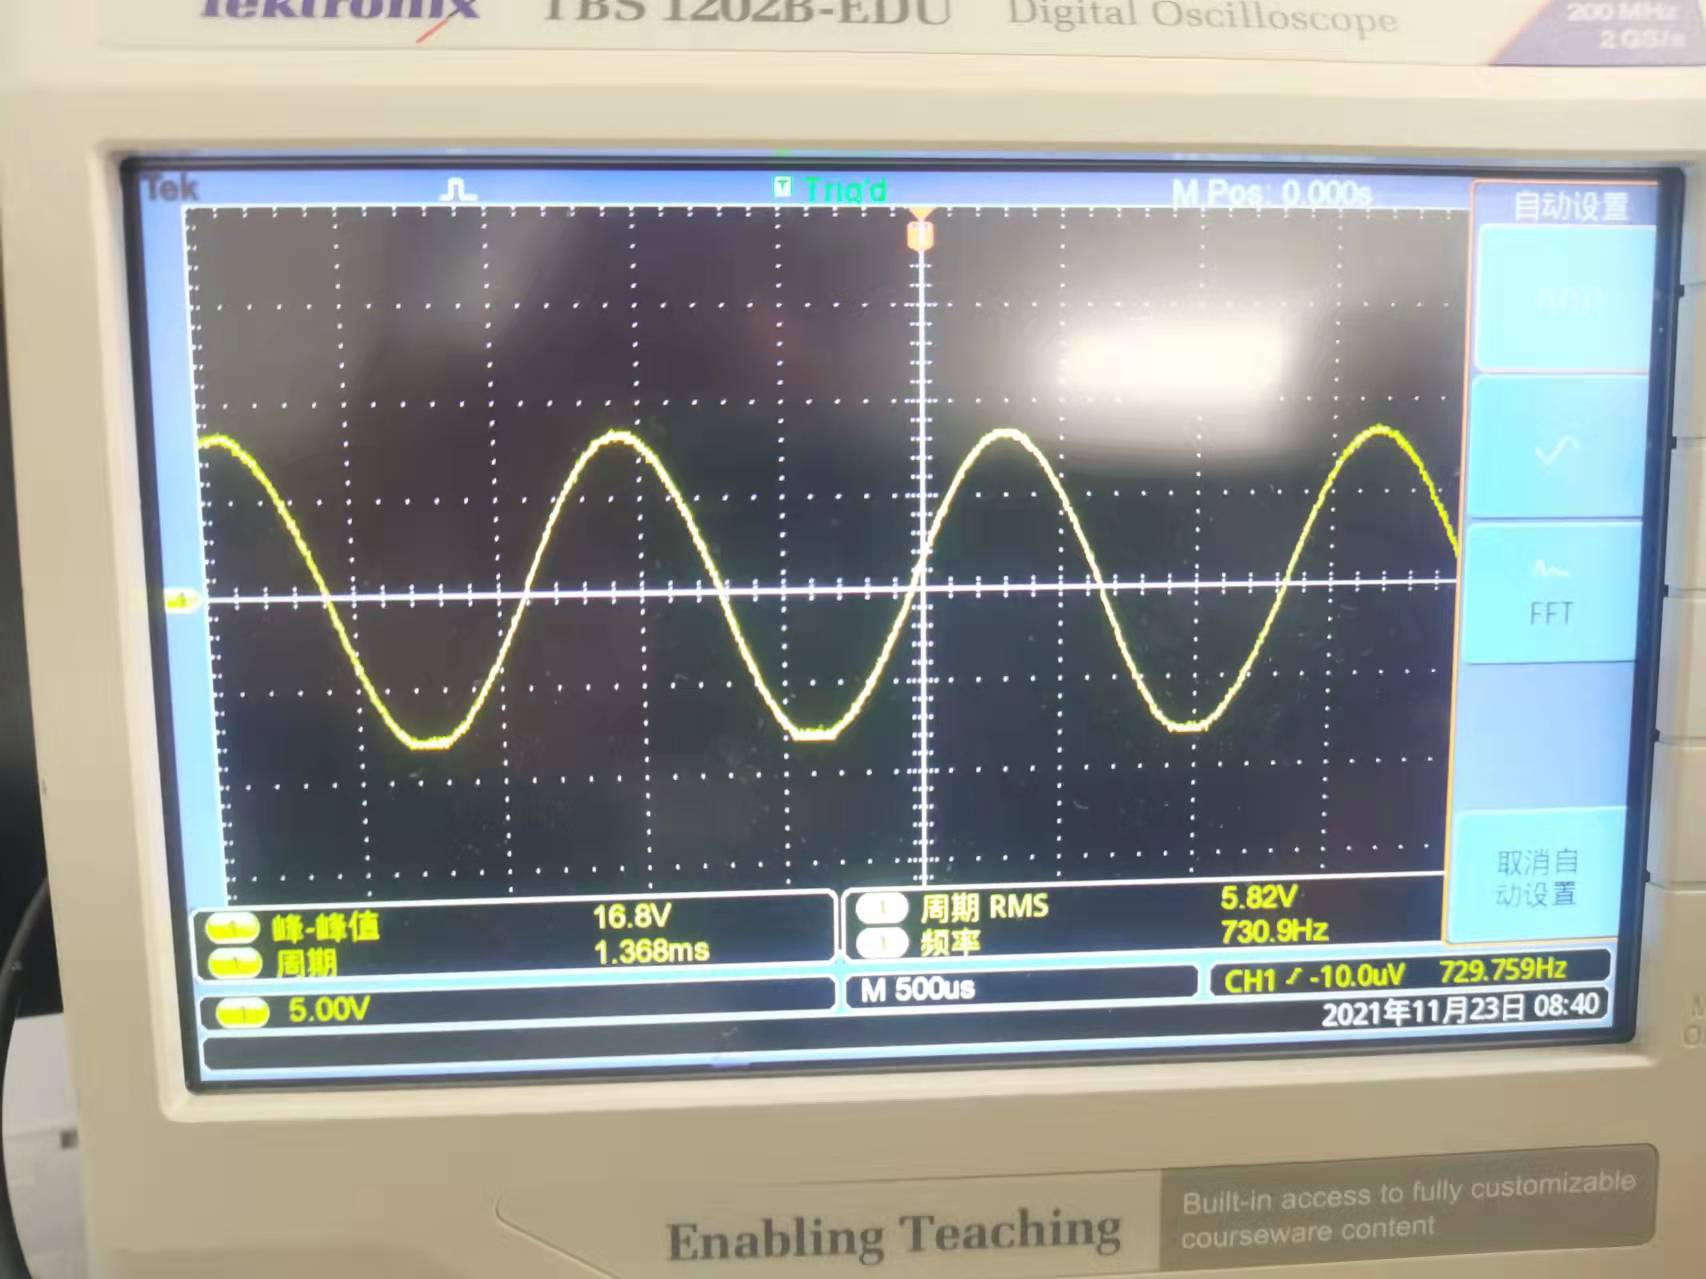
\includegraphics[width = 0.5\textwidth]{1-1-22k-r.jpg}
        \caption{$R=22k \Omega$}
\end{figure}
\begin{figure}[H]
        \centering
        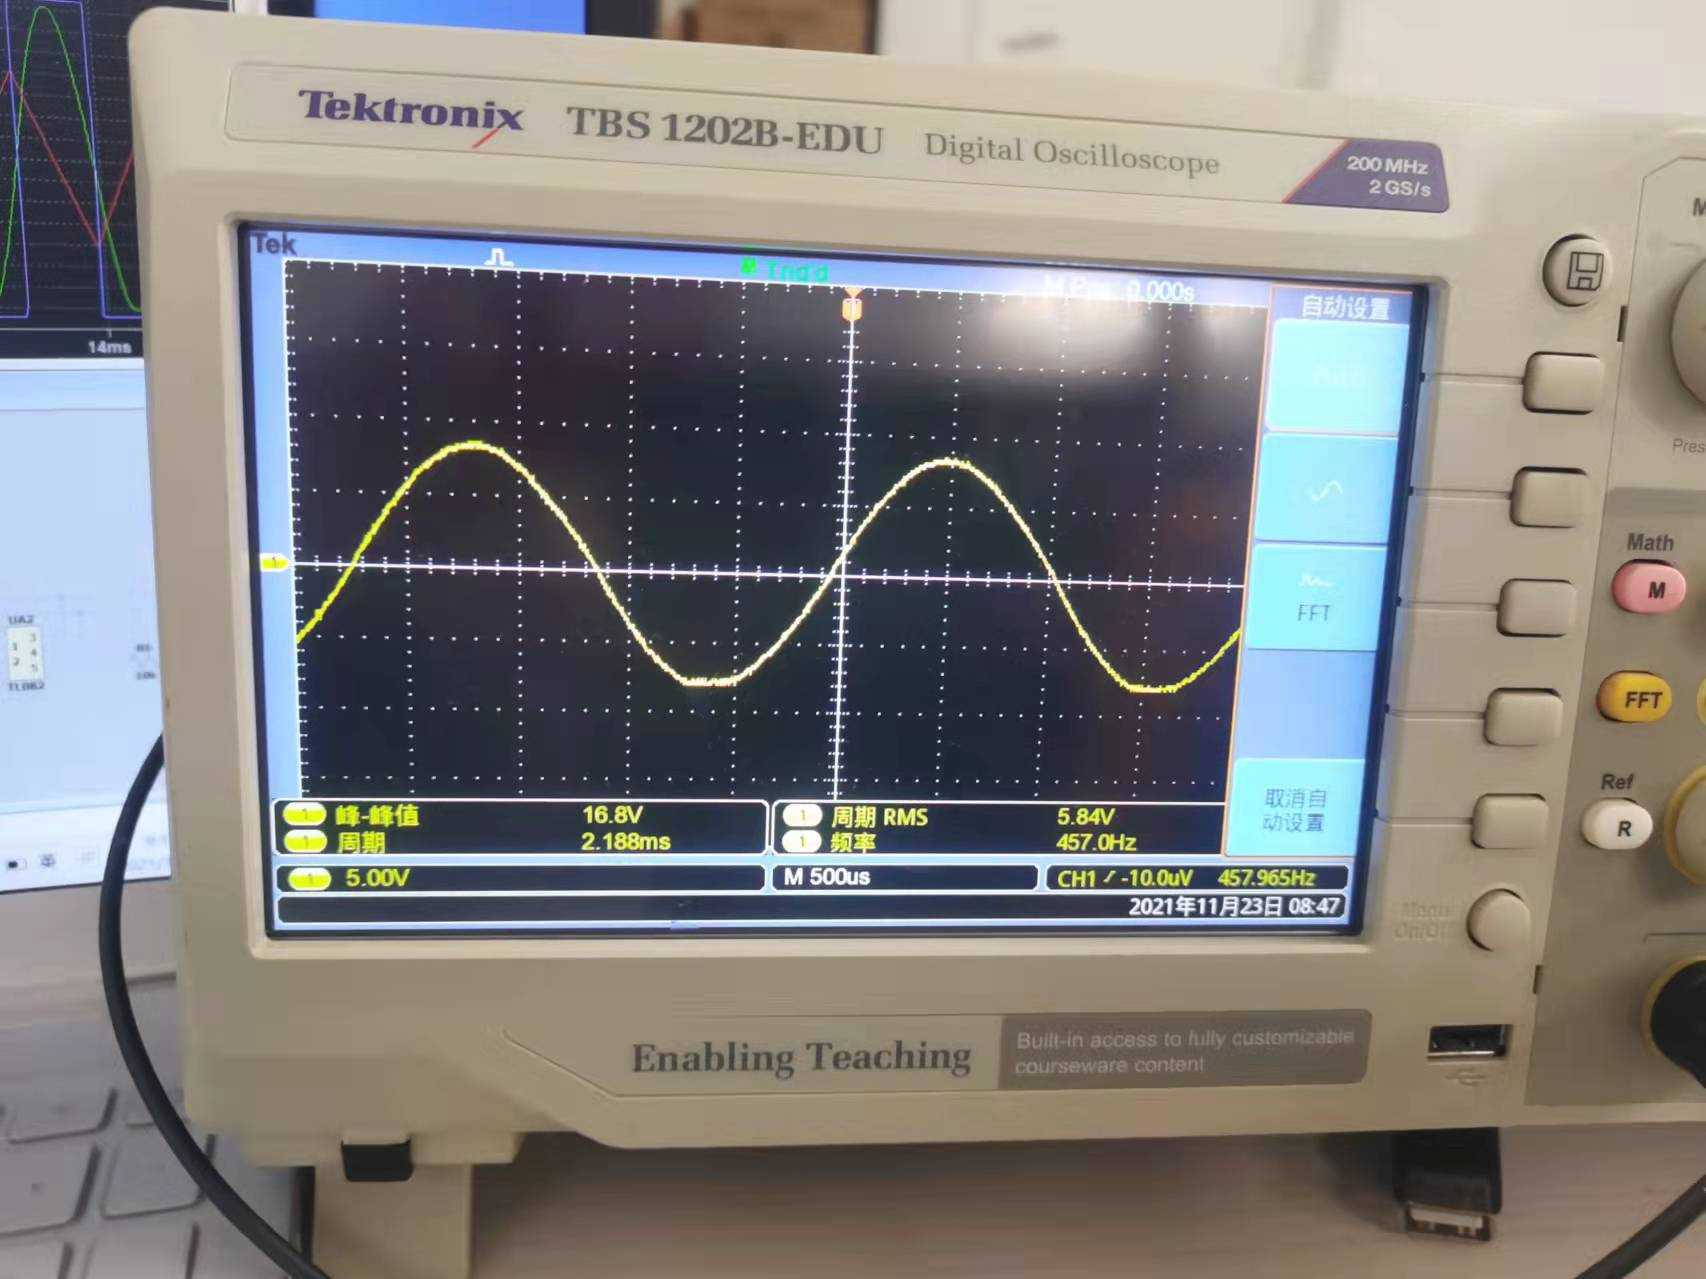
\includegraphics[width = 0.5\textwidth]{1-1-35k-r.jpg}
        \caption{$R=35k \Omega$}
\end{figure}

可以看到频率与理论计算值非常接近。

\subsection*{2、在任务 1 电路的基础上,扩充电路,产生方波和三角波}

采用过零比较器,我们可以将正弦波发生器生成的正弦波转化成方波。

产生方波后,我们在使用积分电路将方波转化成三角波。为了使三角波波形去畸化,
我们在积分电路上并联了一个电阻,便于电容器及时放电。

电路仿真如下:

\begin{figure}[H]
        \centering
        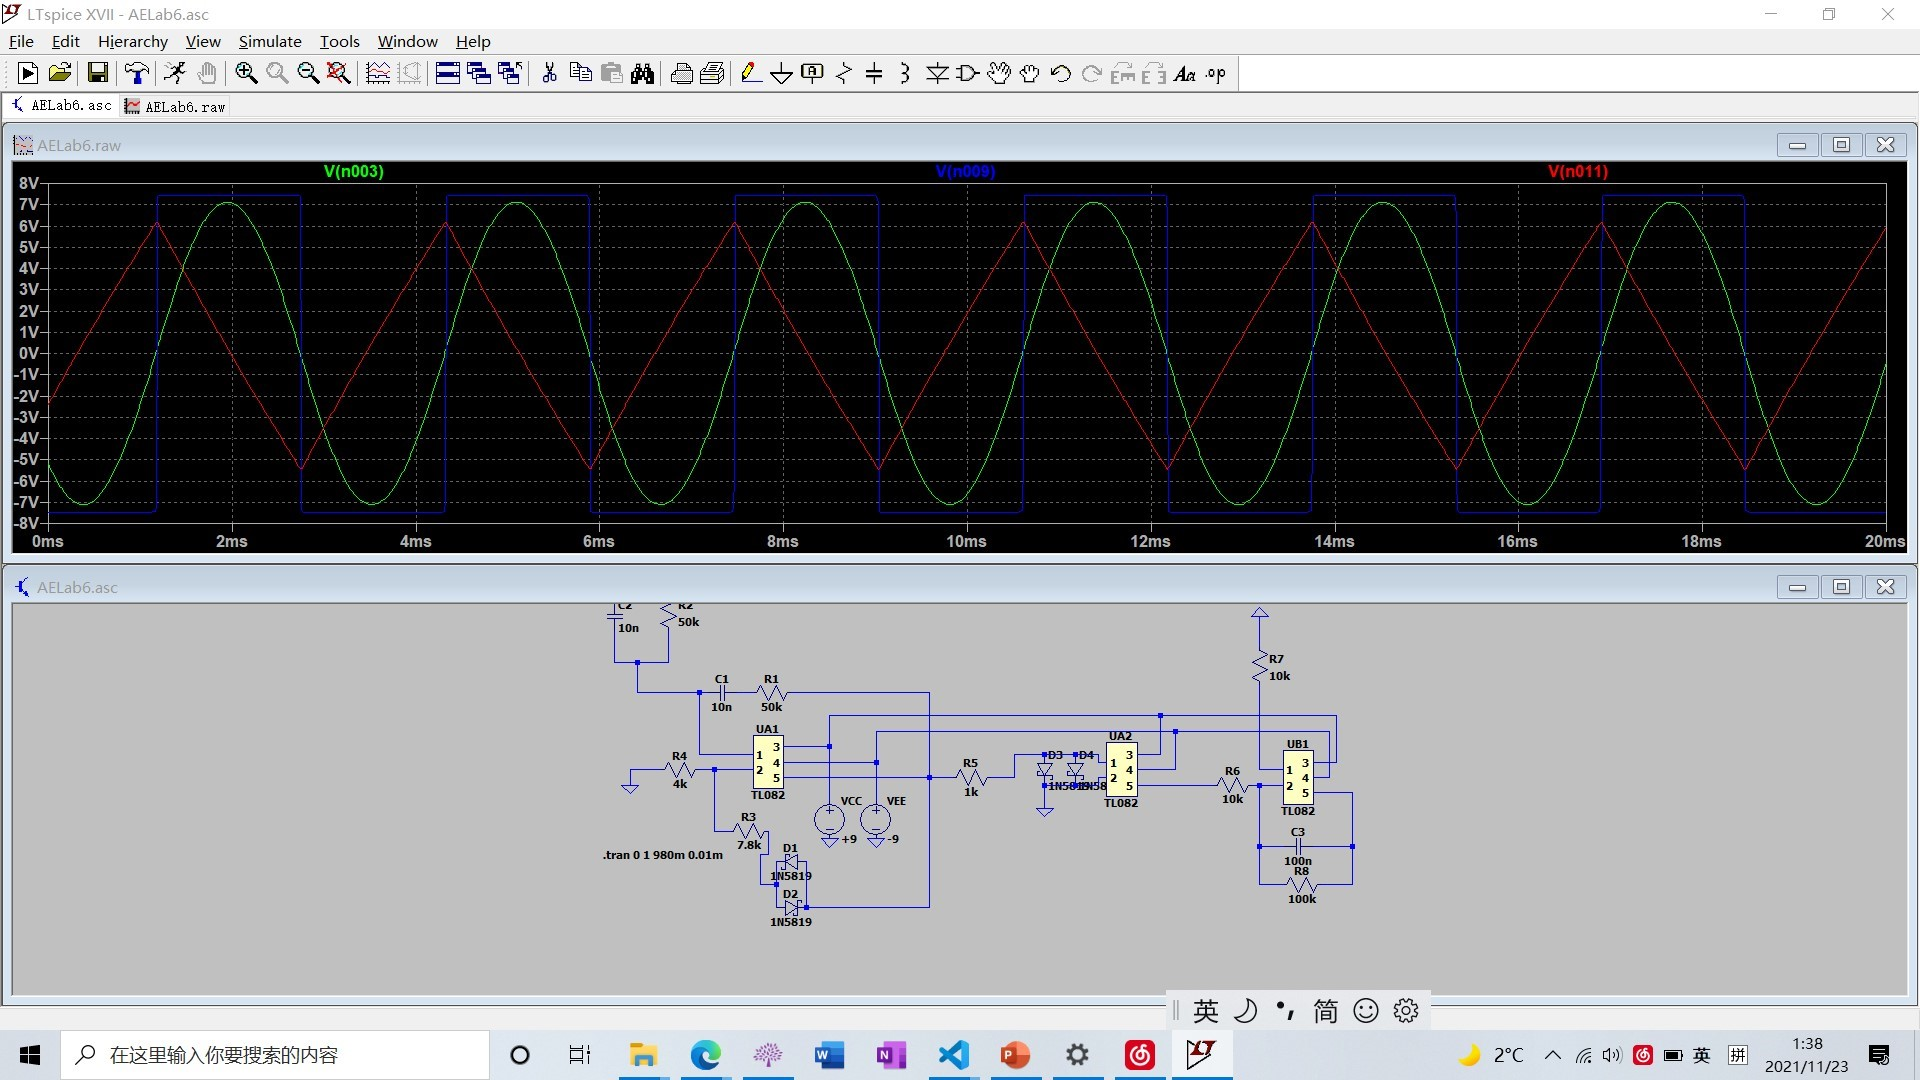
\includegraphics[width =0.7\textwidth]{1-2.jpg}
        \caption{正弦波-方波-三角波发生电路仿真}
\end{figure}

实际搭建电路,得到发生器电路:

\begin{figure}[H]
        \centering
        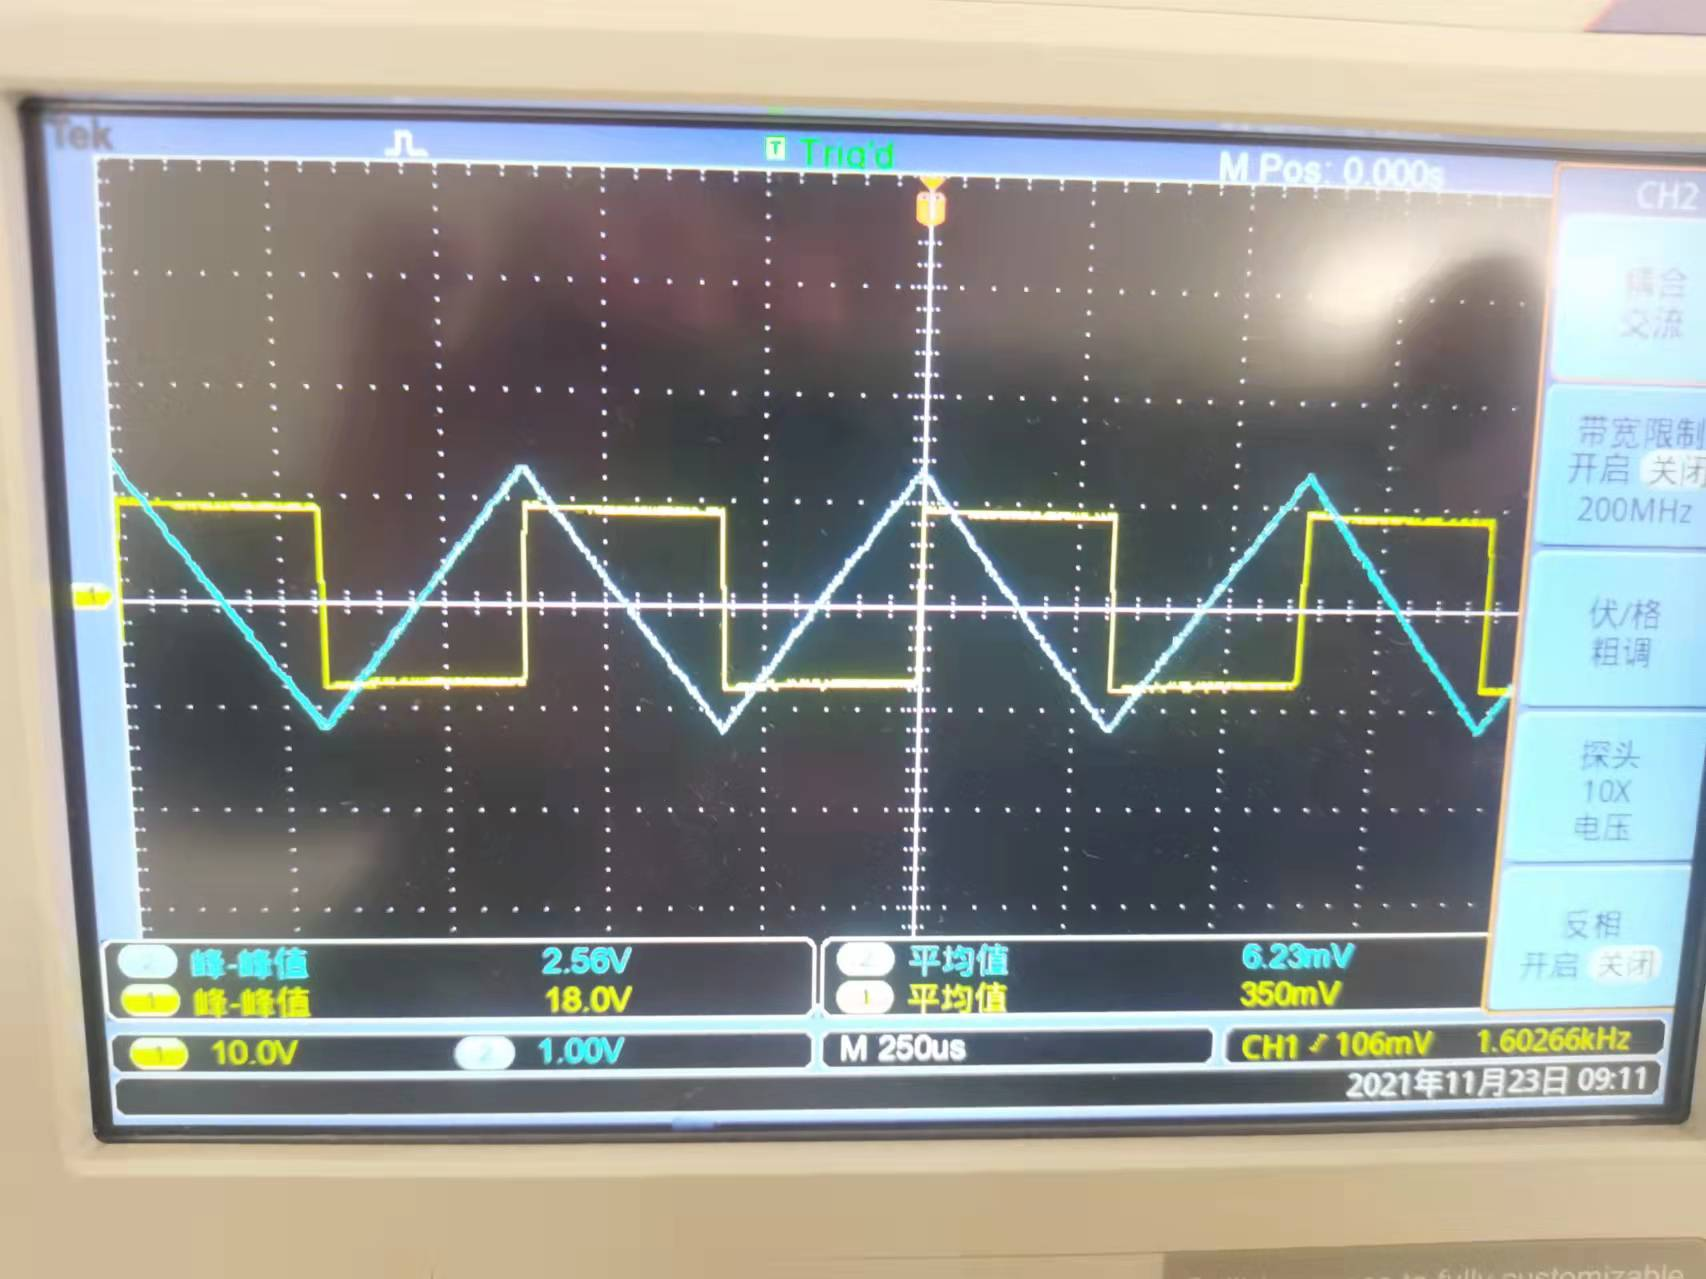
\includegraphics[width =0.7\textwidth]{1-2-total-r.jpg}
        \caption{正弦波-方波-三角波发生电路}
\end{figure}

波形如下图:

\begin{figure}[H]
        \centering
        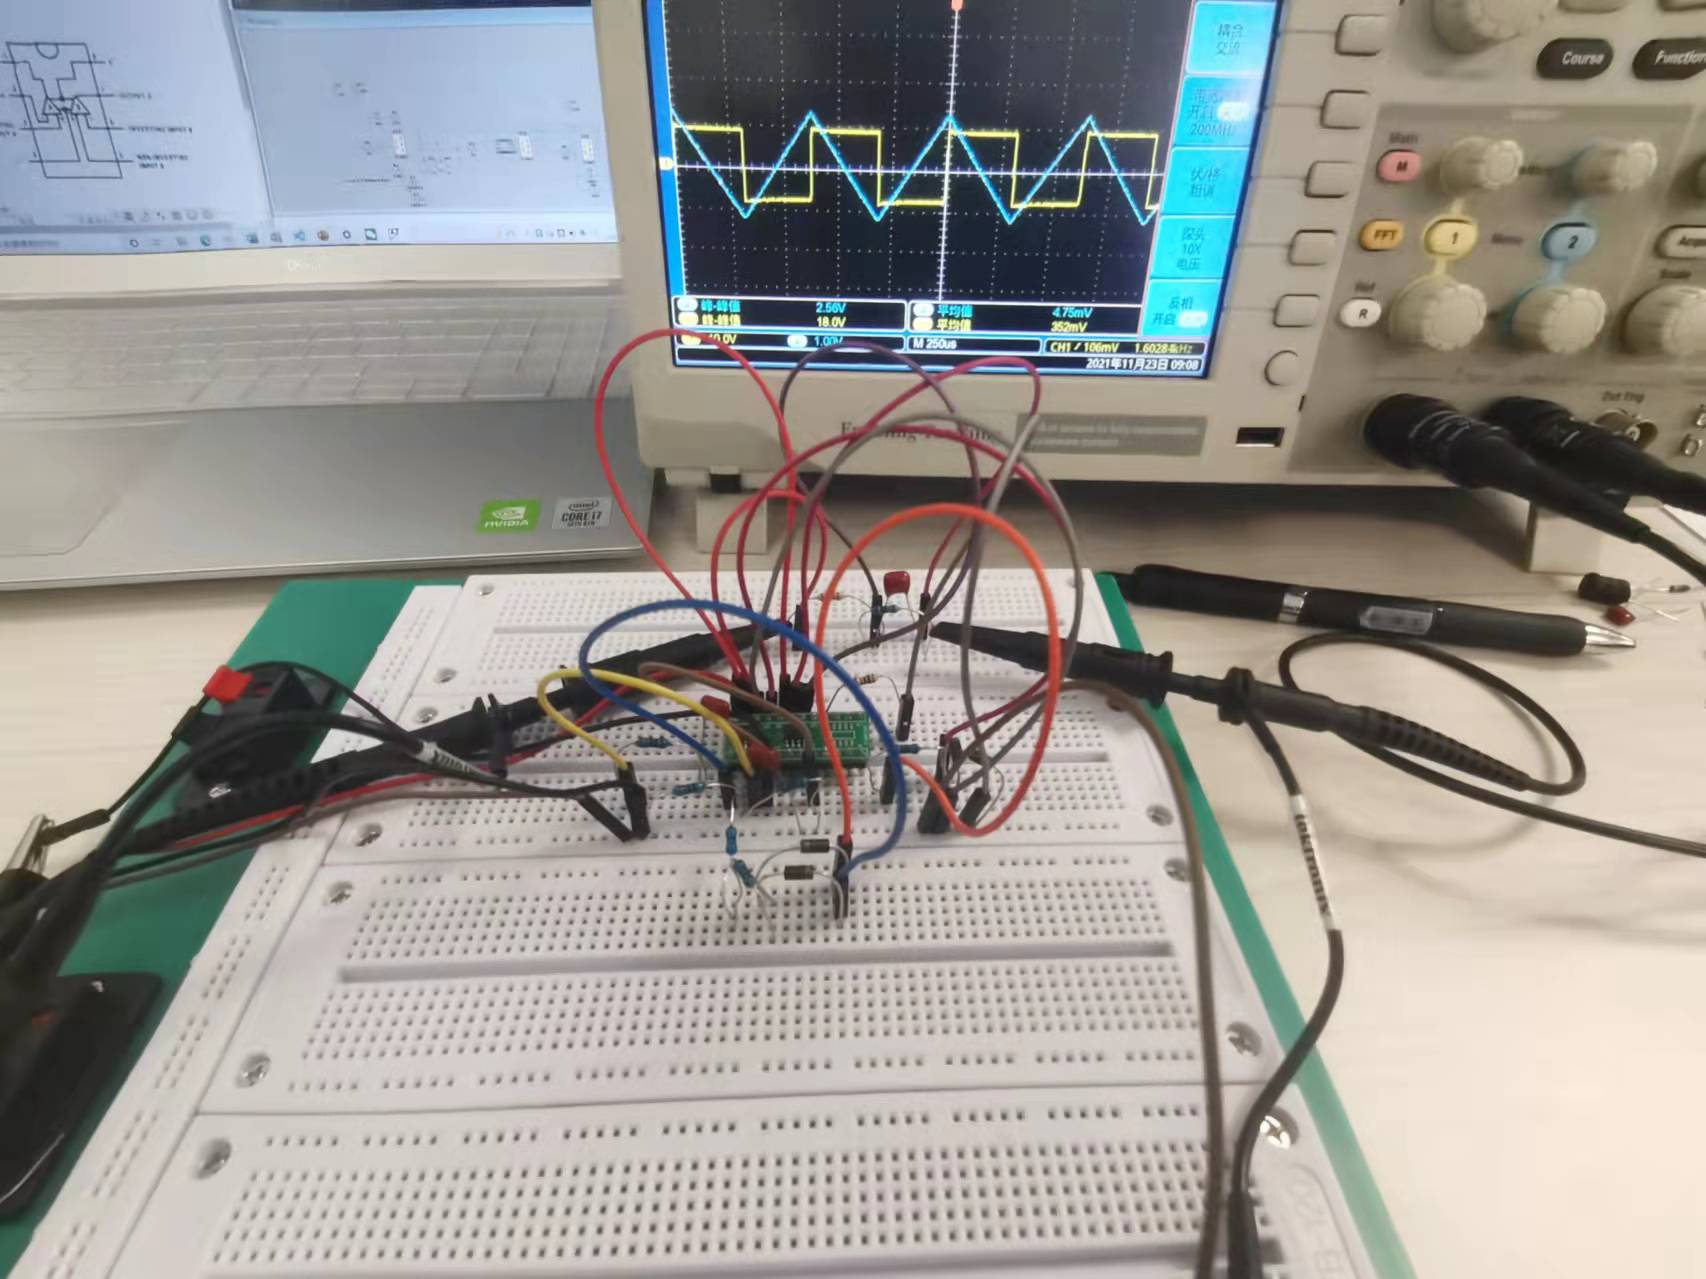
\includegraphics[width =0.7\textwidth]{1-2-r.jpg}
        \caption{正弦波-方波-三角波波形}
\end{figure}

可以看出,三角波、方波、正弦波具有相同的频率。

\subsection*{3、结合仿真与实际测试,分析电路工作原理}

电路的工作原理分析。

正弦波发生电路由一个放大电路和文氏桥选频电路作为反馈电路组成。

文氏桥选频电路的反馈系数为$\hat{F} = \frac{1}{3}$,当放大电路的放大倍数$\hat{A} \approx 3$
的时候,$\hat{F} \hat{A} \approx 1$,相位条件和振幅条件得到满足,回路产生自激振荡产生频率为$1\frac{1}{2 \pi RC}$
的正弦波。

正弦波经过过零比较器,满足$u_i > 0$时$u_0 = U_d$,$u_i < 0$时$u_0 = -U_d$,于是随着正弦波上升过零和下降过零,
在二级电路会输出一个相同频率的方波。

方波转换为三角波采用了积分电路。积分电路满足$u_0 = - \frac{1}{RC} \int u_i  \,dx $。
当$u_i = \pm U_d$的时候,$u_0 =  \mp \frac{1}{RC} U_d t + U_0$产生三角波。


\end{document}